\documentclass[10pt,a4paper]{report}
\usepackage[utf8]{inputenc}
\usepackage[english]{babel}
\usepackage{amsmath}
\usepackage{amsfonts}
\usepackage{amssymb}
\usepackage{graphicx}
\usepackage{hyperref}
\usepackage[autostyle, italian=quotes]{csquotes}
\usepackage[left=2cm,right=2cm,top=2cm,bottom=2cm]{geometry}
\author{Daniele Gilio}
\title{Titanic Logistic Regression}
\graphicspath{ {./images/} }
\begin{document}
\maketitle
\section{Introduction}
In this assignment we were asked to train a logistic regression model in order to predict the survival probability given the following features:
\begin{itemize}
\item Class
\item Gender
\item Age
\item Siblings/Spouses on board
\item Parents and Children on board
\item Passenger Fare
\end{itemize}
The labels associated with those features are binary values indicating whether or not a given passenger survived the disaster. The Training Set is comprised of $710$ samples whereas the Test Set is made of $177$.
\section{Data Analysis}
The first thing we did was an analysis of the data in order to have an idea about how they are distributed and what features might be the most relevant. This was done by plotting the features pairwise and see if a possible decision boundary could be identified. This initial process hinted that the most influential features might be Class and Gender, as we can see in Figure \ref{fig:cvssp}.
\begin{figure}[!ht]
\centering
\includegraphics[width=0.5\linewidth]{{"Class vs. Gender"}.png}
\caption{Class vs. Gender Scatter plot}
\label{fig:cvssp}
\end{figure}
To further investigate this we plotted the \enquote{Empirical} chance of survival, which is basically the data relative frequency, against the features we spotted. The graphs in Figure \ref{fig:emp} tell us that we might be on the right track.
\begin{figure}[!ht]
\centering
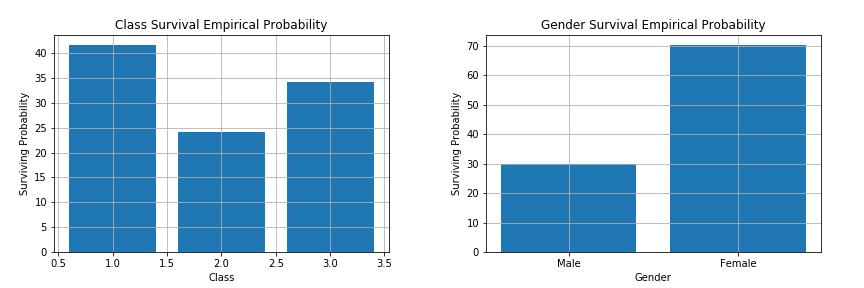
\includegraphics[width=\linewidth]{emp.png}
\caption{Empirical Probabilities for Class (Left) and Gender (Right)}
\label{fig:emp}
\end{figure}
\section{Training}
The training was performed for $2 \cdot 10^5$ steps and we used a Learning Rate equal to $0.001$. Increasing the Learning Rate lead to oscillating values in the loss functions whereas decreasing it worsened the final training loss value and consequently the training accuracy. 
\begin{figure}[!ht]
\centering
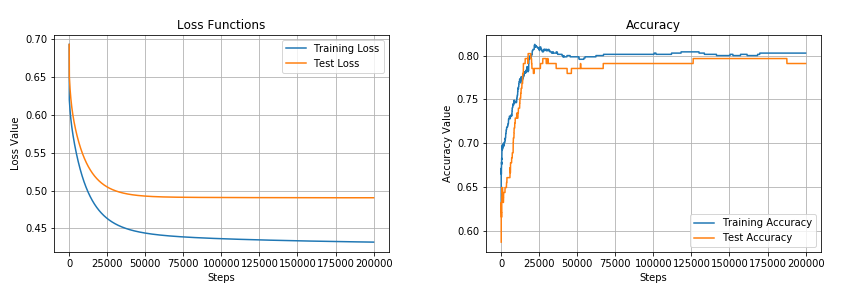
\includegraphics[width=\linewidth]{loss_acc.png}
\caption{Loss (Left) and Accuracy (Right)}
\label{fig:loss_acc}
\end{figure}
The plots in Figure \ref{fig:loss_acc} show both the training and the test loss and their matching accuracy. If we base our model evaluation purely on the loss function, we can say that it may be enough to perform between $5 \cdot 10^4$ and $7.5 \cdot 10^4$ steps to reach convergence as these values are the ones in which the test loss settles on a constant value. Looking at the accuracies though shows that the best step value is probably around $1.5 \cdot 10^5$, because the test accuracy has a peak and it decreases shortly after indicating a possible overfitting issue. The final values for loss functions and accuracies can be found in Table \ref{tab:loss_acc}.
\begin{table}[!ht]
\centering
\begin{tabular}{|l|l|l|}
\hline
         & Training & Test   \\ \hline
Loss     & 0.432    & 0.490  \\ \hline
Accuracy & 80.281   & 79.096 \\ \hline
\end{tabular}
\caption{Losses and Accuracies}
\label{tab:loss_acc}
\end{table}
\section{Model Analysis and Evaluation}
If we take a look at the weights in Table \ref{tab:1}, obtained at the end of the training, we can see that our first intuition was right. Gender is the most influential feature, followed by Class, Siblings/Spouses, Parents and Children, Age and Passenger Fare. We can conclude that the people which were most likely to survive were women travelling alone in first class. The opposite is also true: men in third class travelling with other people were most likely to die. A series of $10^5$ \enquote{Educated Guesses} (Figure \ref{fig:ed_guess}) proves our theory and enlightens the fact the \enquote{Women and Children First} is not a fictional saying but a real world rule of navigation. Given these premises we are glad we were not on the ship since the model predicts a probability of $27.77 \%$ in a best case scenario ($1^{st}$ Class) and a $1.92 \%$ in the worst one ($3^{rd}$ Class).
\begin{figure}[!ht]
\centering
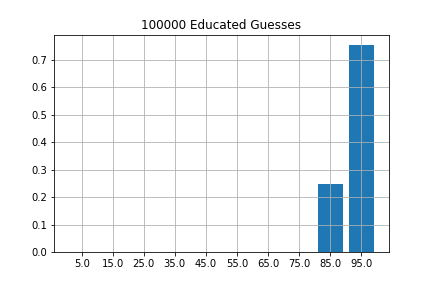
\includegraphics[width=0.5\linewidth]{ed_guess.png}
\caption{\enquote{Educated Guesses}}
\label{fig:ed_guess}
\end{figure}
\begin{table}[!ht]
\centering
\begin{tabular}{|l|c|l|l|l|l|l|}
\hline
        & \multicolumn{1}{l|}{Class} & Gender                     & Age                         & Siblings/Spouses            & Parents/Children            & Fare                       \\ \hline
Weights & -0.974                     & \multicolumn{1}{c|}{2.768} & \multicolumn{1}{c|}{-0.033} & \multicolumn{1}{c|}{-0.302} & \multicolumn{1}{c|}{-0.099} & \multicolumn{1}{c|}{0.003} \\ \hline
Bias    & \multicolumn{6}{c|}{1.56}                                                                                                                                                      \\ \hline
\end{tabular}
\caption{Weights and Bias Table}
\label{tab:1}
\end{table} 
\section{Final Thoughts}
Plotting the contour of decision bound in the Class vs. Gender graph (Figure \ref{fig:conc}) tells us that our model is doing a good job in recognising those two features as the most important ones. In our opinion the model is not overfitting the data since the test accuracy is very close to the training one. Plotting the contour for Class vs. Siblings/Spouses shows, on the other hand, the limitations of the model (Figure \ref{fig:conc}). This is probably due to underfitting, the bias value is in fact rather high compared to the second most influential feature.
\begin{figure}[!ht]
\centering
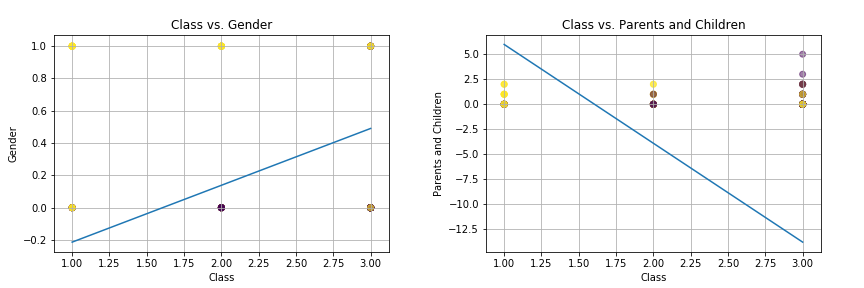
\includegraphics[width=\linewidth]{conc.png}
\caption{Class vs. Gender (Left) and Class vs. Siblings/Spouses (Right). The contours are plotted taking all the non displayed features equal to $0$; it is not ideal but it still works for the purposes of this report.}
\label{fig:conc}
\end{figure}
The model might be improved by adding regularization. We tested both L1 and L2 regularizations with $\lambda=0.005, 0.01, 0.015$. L1 regularization decreased the accuracy by $\sim 0.6 \%$ with $\lambda=0.015$ whereas L2 increased it by $\sim 0.4 \%$. These slight variations in accuracy may indicate that the model is too simple for the problem given, testing a non-linear model might be a better way to represent the data.
\vspace*{\fill}
\\
I affirm that this report is the result of my own work and that I did not share any part of it with anyone else except the teacher.
\\ \\ \\ \\ \\     
\end{document}